{

%fig5 : is separated, back in experiment.tex
\iffalse
\begin{figure*}[!Htbp]

\graphicspath{{fig/}}
    \centering
        \subfigure{ 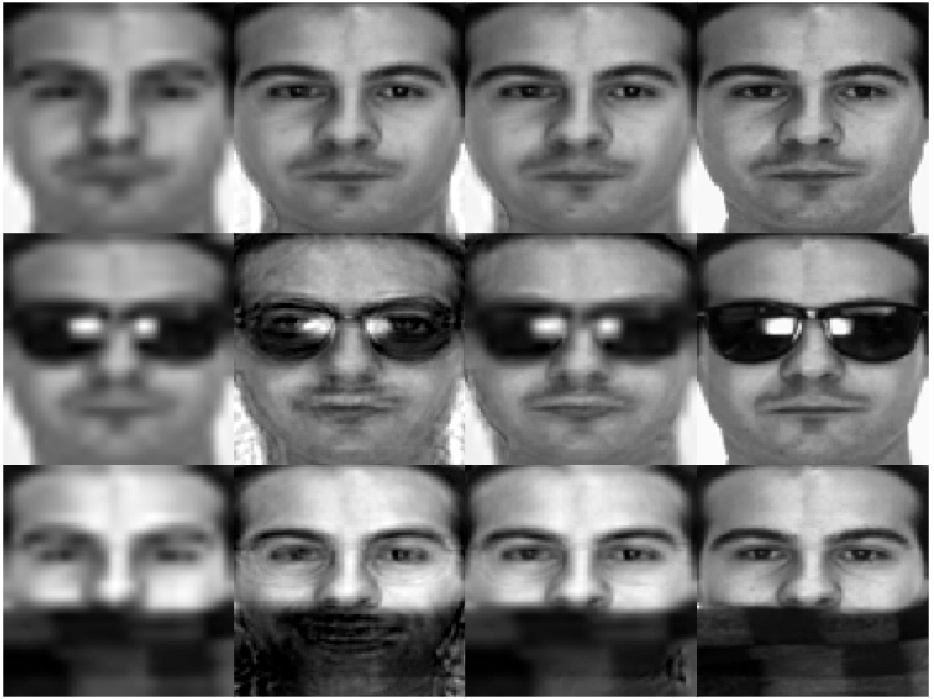
\includegraphics[scale=0.25]{exp_ori.jpg}}
        \subfigure{ 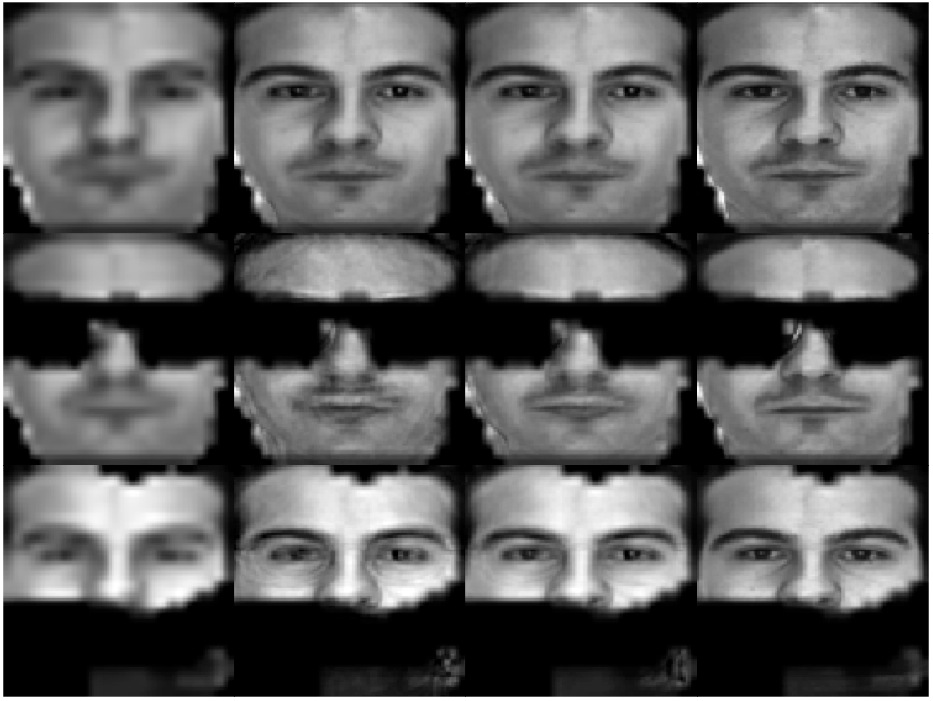
\includegraphics[scale=0.25]{exp_masked.jpg}}
    \caption{The hallucination result of experiment. The columns in each side are (a) Bicubic (b) Jung's Method \cite{convex}, (c) our proposed method, and (d) ground truth respectively\label{fig:exp}}
\end{figure*}
\fi

With the proposed occlusion invariant sparse coding scheme in Section~\ref{subsec:aRSC}, we are able to derive the sparse coefficients for representing the LR input $\by_L$ using LR dictionary $\bD_L$. To predict the corresponding HR output image, we apply the sparse representation based super resolution techniques of~\cite{TIP10,convex} for our face hallucination task, as we now discuss.

Given the LR dictionary and its corresponding HR version $\bD_H\in\Real^{m\times n}$, it is assumed in~\cite{TIP10,convex} that the sparse coefficients for representing the HR image $\by_H\in\Real^m$ would be identical to those for its LR input $\by_L\in\Real^d$. However, since approaches like~\cite{TIP10,convex} are not robust to occluded regions, we need to apply the proposed occlusion invariant sparse coding scheme for addressing this challenging problem.

Recall that, in Section~\ref{subsec:aRSC}, our proposed algorithm is able to derive the weighting matrix $\bW_L$ from $\by_L$ and $\bD_L$, which indicates and recovers the non-occluded image regions while suppressing corrupted pixels. For hallucinating the HR image, we first extend the derived matrix $\bW_L$ to $\bW_L\in\Real^{m\times m}$ via interpolation. Next, we consider patch-based sparse representation for performing occlusion invariant face hallucination. That is, we divide the LR input $\by_L$ into overlapping patches, denoted by $\by_L^i$, where $i$ is the patch index. Similary, each LR training image in $\bD_L$ is also divided into overlapping patches, denoted by $\bx_{L,j}^i$ for $j=1, 2,~\ldots, N$. 

Now, the sparse coefficient for the $i$th patch can be determined by solving the following problem:
\begin{equation}\label{eqn1}
     \min_{\balpha_L^i} \norm{\bW_L^i(\by_L^i - \bD_L^i\balpha_L^i)}_2^2+\lambda\norm{\balpha_L^i}_1,
\end{equation}
where $\bW_L^i$ indicates the $i$th patch of $\bW_L$. With $\balpha_L^i$ calculated, the $i$th output patch can be derived~by
\begin{equation}
\by_H^i = \bW_H^i\bD_H^i\balpha_L^i,
\end{equation}
where $\bW_H^i$ is the $i$th patch in $\bW_H$, and $\bD_H^i$ indicates the $i$th patches of $\bD_H$. Once all the patches for the HR output is obtained, hallucination of $\by_H$ is complete. We note that, for occluded image regions in $\by_H$, we simply perform bicubic interpolation on the associated regions of the LR input. The framework of our method is depicted in Figure~\ref{fig:algFlow}.

}


%\mathop{\arg\min}_\limits{w_{m}(i,j)}
